% !TeX root = ../main.tex
\begin{cnabstract}
本文复现申万宏源的柏顿·墨基尔选股法，并检验在保留持续盈余成长与低估值框架后，两种选股改进及其仓位规则如何改变组合表现。基于 CSMAR 数据，本文构建候选池三因子排序与波动率目标仓位、核心优先补位与均线趋势风控两条路线，分别以未控仓组合衡量仓位规则的影响。2003 年 4 月至 2015 年 6 月，基础复现的年化收益为 38.86\%，月末最大回撤幅度为 70.11\%。2015 年 8 月至 2026 年 9 月的共同延展期内，基础策略年化收益为 14.10\%，两种未控仓选股组合分别为 18.99\% 和 16.83\%。在三因子组合上按波动率调整仓位，年化收益降至 16.68\%，最大回撤幅度维持在 29.42\%。在补位组合上叠加均线规则，年化收益为 9.00\%，最大回撤幅度从 26.65\% 收窄至 15.98\%。按实际财报公告日重算后，补位组合在 2021 年以来的年化收益从 21.97\% 降至 8.62\%。历史结果显示，评价仓位规则应同时考虑底层选股、样本窗口和财务信息时点。
\end{cnabstract}
\cnkeywords{墨基尔选股法；盈余成长；低市盈率；波动率目标；趋势风控}

\section{引言}

高收益的选股规则可以伴随很深的回撤。陈杰（2015）将柏顿·墨基尔的持续成长与合理估值理念用于 A 股，在原报告样本中获得 36.74\% 的年化收益，同时经历 70.19\% 的最大回撤\cite{chen2015}。延长样本后，两个问题尤其值得检验。持续成长门槛和低估值交集可能使候选过少，改用补位或多维排序能否提高组合收益？给定选股名单，连续调整仓位与按趋势持股或持现，分别改变了多少收益和回撤？

Fama 和 French（1992）发现规模与账面市值比有助于解释股票平均收益的截面差异\cite{ff1992}。Asness 等（2013）记录了价值和动量在多个市场中的收益规律，为在估值筛选后利用价格趋势提供了经验背景\cite{amp2013}。Faber（2007）的月度均线模型为根据指数趋势在风险资产与现金之间切换提供了可检验的规则\cite{faber2007}。本文沿着两条思路展开。一条在成长与估值候选池中加入盈利质量、动量和规模排序，再以组合历史波动控制仓位。另一条优先保留符合严格条件的核心股票，再用指数均线决定组合是否持仓。

本文将策略对照分成两层。第一层以同一基础规则衔接原研报复现和后续延展。第二层在每条路线内固定选股名单，成对比较加入仓位规则前后的业绩，再对两套完整方案使用相同的 134 个月评价窗口。这样的设计使选股规则与仓位规则各自的比较对象明确，并允许用长样本检验风控表现是否随窗口变化。

\section{数据与变量}

本文使用 CSMAR 的 A 股月度行情、月末总市值、季度累计总净利润、财报公告日期和上证综指日行情。估值截面覆盖证券代码以 0、3、6 开头的股票。基础版与路线一的月收益沿用市场类型 1、4、16，路线二另纳入类型 32 的科创板收益。实证部分另将路线二的股票收益覆盖统一至 1、4、16。个股收益含现金红利再投资，上证综指基准由价格指数日收益逐月复利。

同比成长率以本期累计总净利润除以上年同期累计总净利润，再减 1。上年同期利润非正或缺失时，该期没有有效成长率。非年报的滚动四季利润等于上年全年利润加本年累计利润、减上年同期累计利润。年报直接使用当年全年利润。用调仓月末总市值除以滚动四季利润得到市盈率，最终入选股票的市盈率须为正。

月频复现的实际持有期为 2003 年 4 月至 2015 年 6 月。研究以 2015 年 8 月至 2026 年 9 月为共同延展窗口，避开原研报收益统计截至 2015 年 7 月的区间。样本起点前的财务、价格和持仓历史用于形成信号。主表从共同窗口起点重新计算净值和回撤。

\section{研究设计}

\subsection{基础复现与同规则延展}

基础复现 F 使用固定的季度末信号。成熟期要求最近 20 个季度齐全且成长率均为正，再取当期成长率前 30\% 与市盈率最低 30\% 的交集。两项排名分别使用有效观测的全截面。有限负市盈率先参与排序，再剔除非正市盈率。2003 至 2007 年的初始期要求已观察到的成长历史连续且均为正，通过估值筛选后按成长率选取最多 15 只。延展 E 保留同一套规则，把最后持有月份推进至 2026 年 9 月。

\subsection{路线一：候选池三因子排序与波动率目标仓位}

P1 在成熟期要求最近 20 季齐全且至少 19 季成长率为正，成长率和市盈率在历史达标且两项指标有效的候选池内排序。先按两榜前 30\% 定义核心候选，再将门槛放宽至前 50\% 形成扩展池，两池均要求持仓市盈率为正。以最近最多 20 期累计净利润的正值占比、调仓月之前 12 个月的累计收益（至少 8 个月有效）和较小市值衡量质量、动量与规模。三项在同一候选池中转换为方向一致的百分位，等权计分，核心与扩展候选按分数合并选取最多 15 只。

P3 沿用 P1 的股票名单。每月月初根据过去最多 12 个月的 P1 净收益估计年化波动率 $\widehat{\sigma}_{t-1}$，历史至少有 6 个月且波动率有效时，将仓位设为 $\min\{1,0.20/\widehat{\sigma}_{t-1}\}$，否则维持满仓。若月初组合净值较本季度起点下跌至少 25\%，当季余期持现。P3 按仓位缩放 P1 当月净收益，现金收益计零。

\subsection{路线二：核心优先补位与均线趋势风控}

B 同样容许最近 20 季中出现一次非正成长，但还要求当期成长率为正。成长率在有有效成长率的全截面排序，市盈率在正市盈率股票中排序。两项名次同时满足前 30\% 的股票进入核心池，组合不足 15 只时再从同时满足前 50\% 的候选补位。核心和补位池分别按两项名次占各自榜单总数的比例之和由小到大取股。

C 沿用 B 的选股名单。上月末上证综指收盘价达到当时 10 个月简单移动均线，本月持有该组合。低于均线时持有现金，收益计零。趋势信号每月更新，股票名单仍由季度信号决定。

\subsection{收益、费用与比较方法}

组合从信号次月起持有三个月，每月对有有效收益的持仓再等权。基础策略及两种选股组合在有持仓的季度首月固定扣 0.13\%。C 在持仓开关变化时也扣 0.13\%，与季度调仓重合时合并为一次。P3 直接缩放底层净收益，仓位调整没有另计费用。各方案共同采用月收益复利计算年化收益，以月收益标准差乘 $\sqrt{12}$ 计算年化波动，以零无风险利率计算年化夏普比率。最大回撤基于含初始净值 1 的月末序列，表中以损失幅度正值报告。

\section{实证结果}

\subsection{原研报区间复现}

基础复现覆盖 147 个月，年化收益 38.86\%，最大月末回撤幅度 70.11\%，相应的上证综指年化收益为 9.09\%。原研报公布年化收益 36.74\%、最大回撤幅度 70.19\%。两项统计均反映了高历史收益伴随较大峰谷损失的特征。原研报按财报发布安排调仓并采用日频回测，收益统计截至 2015 年 7 月。本文按固定季度末形成名单，持有收益截至 2015 年 6 月，因此两组数字的比较需要同时考虑调仓时点、观察频率和样本末月。基础复现 F 与延展 E 在 147 个共同月份的组合收益逐月一致。

\Needspace{13\baselineskip}
\subsection{共同延展区间的收益与回撤}

\begin{table}[H]
\centering
\caption{共同延展区间的绩效，2015 年 8 月至 2026 年 9 月}
\label{tab:main}
\small
\renewcommand{\arraystretch}{1.2}
\begin{tabular}{@{}lrrrr@{}}
\toprule
方案 & 年化收益（\%） & 年化波动（\%） & 最大回撤（\%） & 夏普比率 \\
\midrule
E 基础延展 & 14.10 & 27.81 & 33.15 & 0.610 \\
P1 候选池三因子 & 18.99 & 21.24 & 29.42 & 0.930 \\
P3 波动率目标仓位 & 16.68 & 18.69 & 29.42 & 0.922 \\
B 核心优先补位 & 16.83 & 22.32 & 26.65 & 0.811 \\
C 均线趋势风控 & 9.00 & 14.41 & 15.98 & 0.669 \\
上证综指 & 0.35 & 16.90 & 32.50 & 0.106 \\
\bottomrule
\end{tabular}

\medskip
\begin{minipage}{0.95\linewidth}\footnotesize
注：每个方案均为 134 个月，夏普比率按零无风险利率计算。资料来源：CSMAR，作者计算。
\end{minipage}
\end{table}

表\ref{tab:main}显示，P1 和 B 的年化收益分别较基础延展高 4.90 和 2.73 个百分点，月末最大回撤幅度均小于基础策略。在两条路线内部，P3 的年化波动由 21.24\% 降至 18.69\%，最深回撤幅度同为 29.42\%。C 的最大回撤幅度较 B 收窄 10.67 个百分点，年化收益减少 7.83 个百分点。P3 的收益和夏普高于 C，而 C 的最大回撤较小。两套完整方案的差异同时包含底层选股和仓位规则。

\begin{figure}[!t]
\centering
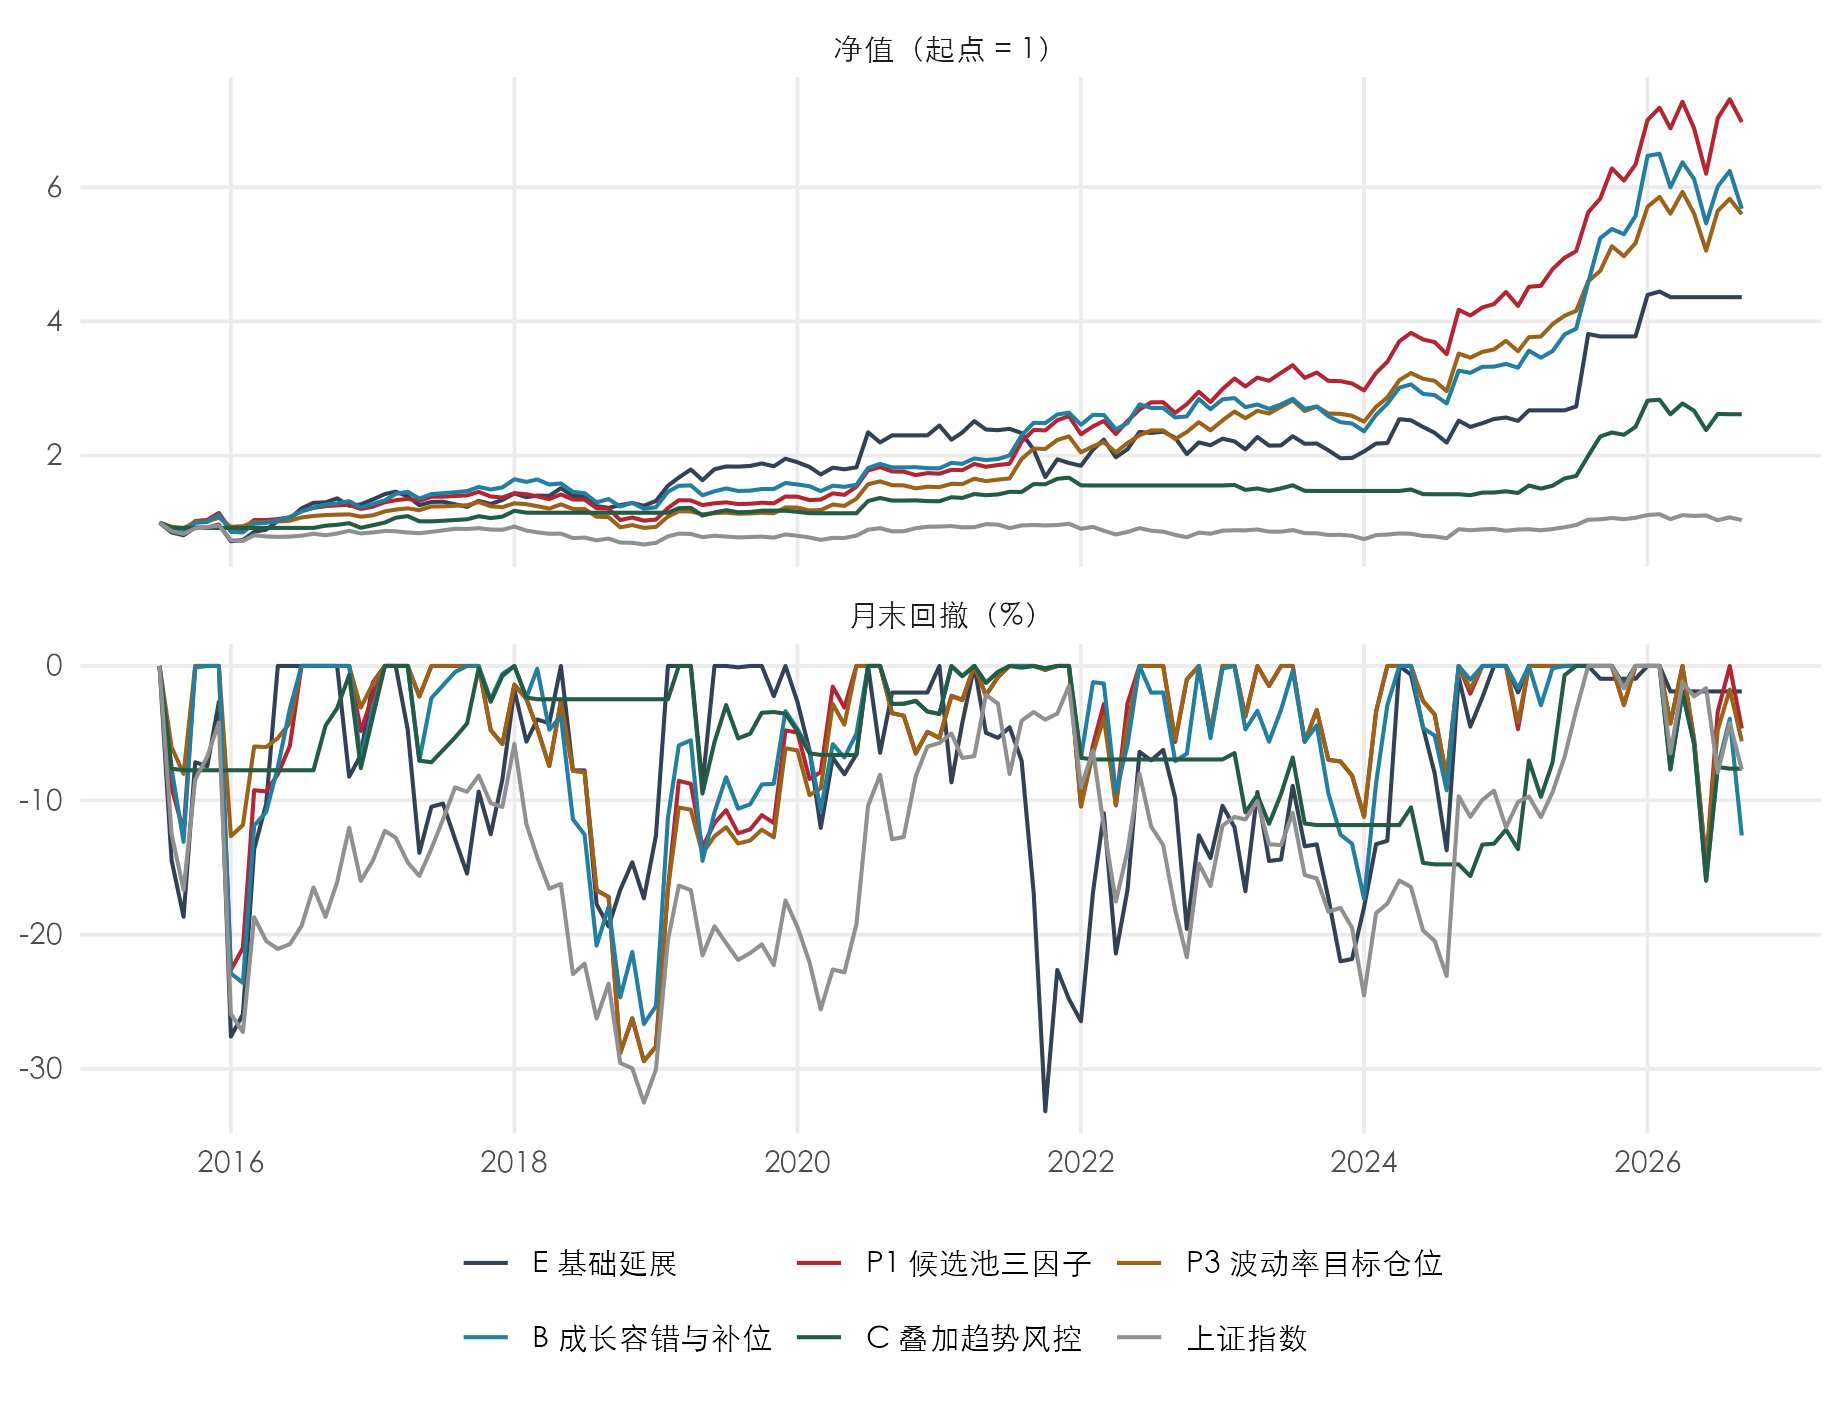
\includegraphics[width=0.9\linewidth]{figures/two-routes.png}
\caption{共同延展区间的组合净值与月末回撤}
\label{fig:routes}
\begin{minipage}{0.95\linewidth}\footnotesize
注：净值在 2015 年 8 月首笔收益前设为 1。回撤从各组合已实现的历史净值高点计算。资料来源：CSMAR，作者计算。
\end{minipage}
\end{figure}

\subsection{仓位机制与窗口差异}

在共同延展期内，P3 的平均仓位为 89.62\%，零仓位月份为零。P3 的风险变化来自波动目标下的仓位缩放。将观察窗口延长到 2003 年 4 月至 2026 年 9 月，P3 相对 P1 的最大回撤幅度从 68.87\% 收窄至 32.74\%，年化收益从 29.64\% 降至 23.19\%。长区间与延展区间的差异表明，波动率控仓对最深历史回撤的影响与纳入的下跌阶段有关。

C 在共同延展期内有 56\ 个零仓位月份，平均仓位为 58.21\%。月度趋势开关减少了组合暴露，也减少了对持现月份上涨的参与。图\ref{fig:routes}把这种权衡表现在净值与回撤两条路径上。相比单列一个全期夏普比率，成对结果更直接地说明了两条仓位规则在何处改变风险和收益。

\subsection{公告日、时间切分与收益覆盖}

报告期口径将财务数据映射到季度末。为考察信息时点，本文在路线二中按实际公告日期重新形成截面，要求当期财报以及同比、TTM 和成长历史所依赖的报表均在调仓前公告，并在距调仓日一年内的可用财报中选取最新一期。计算仍使用数据库当前记录的会计数值。表\ref{tab:ann}显示，在 2021 年 1 月至 2026 年 9 月，B、C 在公告日口径下的年化收益分别为 8.62\% 和 7.23\%，同期基础策略为 $-18.37\%$。B 和 C 在该口径下仍优于同期基础策略，但收益水平对财务信息时点敏感。表中公告日结果的范围为路线二及其基础对照。

\begin{table}[htbp]
\centering
\caption{路线二的公告日敏感性，2021 年 1 月至 2026 年 9 月}
\label{tab:ann}
\small
\renewcommand{\arraystretch}{1.2}
\begin{tabular}{@{}lrrrr@{}}
\toprule
& \multicolumn{2}{c}{报告期口径（\%）} & \multicolumn{2}{c}{公告日口径（\%）} \\
\cmidrule(lr){2-3}\cmidrule(l){4-5}
方案 & 年化收益 & 最大回撤 & 年化收益 & 最大回撤 \\
\midrule
基础策略 & 11.76 & 33.15 & $-18.37$ & 72.27 \\
B 核心优先补位 & 21.97 & 17.34 & 8.62 & 31.71 \\
C 均线趋势风控 & 12.61 & 15.98 & 7.23 & 24.56 \\
\bottomrule
\end{tabular}

\medskip
\begin{minipage}{0.95\linewidth}\footnotesize
注：每组 69 个月。公告日重算会同时改变可用报告期和候选截面。资料来源：CSMAR，作者计算。
\end{minipage}
\end{table}

按 2015 年 8 月至 2020 年 12 月的夏普比率从路线二预设候选中选择，前段胜出的是基础策略，其后段年化收益为 11.76\%。B 的后段收益较高，属于历史候选的并列比较。另将 B、C 的收益覆盖统一至路线一的市场类型，年化收益分别约为 16.9\% 和 9.0\%，主表中两条路线的收益与回撤排序保持一致。

\section{结论}

以同规则延展为基准，候选池三因子排序和核心优先补位在 2015 年 8 月至 2026 年 9 月均提高了历史年化收益。给定选股名单，波动率目标仓位在长样本中收窄了历史最深回撤，在共同延展期则主要体现为较低波动。均线趋势风控在共同窗口中将最大回撤幅度从 26.65\% 降至 15.98\%，代价是更低的复利收益。

这两条路线分别展示了连续缩放风险暴露和按趋势切换风险暴露的组合结果。对选股收益的判断则需要同时考察财务信息时点。公告日重算后，路线二与基础策略的相对排序得到保留，绝对收益随可用财务截面变化而下降。两组证据分别回答了仓位如何改变回撤，以及选股收益对财报可用时间有多敏感。

\renewcommand{\bibname}{参考文献}
{\let\chapter\section
\begin{thebibliography}{9}
\bibitem{chen2015} 陈杰. 柏顿·墨基尔成功选股法：申万大师系列·价值投资篇之十二[R]. 申万宏源研究, 2015-10-14.
\bibitem{ff1992} Fama E F, French K R. The cross-section of expected stock returns[J]. The Journal of Finance, 1992, 47(2): 427--465. \href{https://doi.org/10.1111/j.1540-6261.1992.tb04398.x}{DOI}.
\bibitem{amp2013} Asness C S, Moskowitz T J, Pedersen L H. Value and momentum everywhere[J]. The Journal of Finance, 2013, 68(3): 929--985. \href{https://doi.org/10.1111/jofi.12021}{DOI}.
\bibitem{faber2007} Faber M T. A quantitative approach to tactical asset allocation[J]. The Journal of Wealth Management, 2007, 9(4): 69--79. \href{https://mebfaber.com/2009/02/19/a-quantitative-approach-to-tactical-asset-allocation-updated/}{作者页面}.
\end{thebibliography}}
